\documentclass[fontsize=11pt,a4paper,oneside,parskip=half,
 headings=normal,captions=tableheading]{scrartcl}

\usepackage[utf8]{inputenc}
\usepackage[T1]{fontenc}
\usepackage[brazilian]{babel}
\usepackage{lmodern}
\usepackage{tgheros}
\ifdefined\pdfmapfile\pdfmapfile{+qhv.map}\fi
\renewcommand{\familydefault}{\sfdefault}
\usepackage{microtype}
\usepackage[margin=22mm,headheight=16pt,headsep=7mm,footskip=11mm]{geometry}
\usepackage{graphicx}
\usepackage{pdflscape}
\usepackage{float}
\usepackage{booktabs}
\usepackage{tabularx}
\usepackage{longtable}
\usepackage{array}
\usepackage{enumitem}
\usepackage[table]{xcolor}
\usepackage{scrlayer-scrpage}
\usepackage{hyperref}
\usepackage{bookmark}

\definecolor{navy}{HTML}{1A2B3D}
\definecolor{accent}{HTML}{176B83}
\definecolor{muted}{HTML}{586777}
\definecolor{paperblue}{HTML}{EDF3F7}
\definecolor{tableline}{HTML}{D6E0E7}
\hypersetup{colorlinks=true,linkcolor=accent,urlcolor=accent,
 pdftitle={Cadastro de Currículos -- Implementação do desafio CIEE/PR},
 pdfauthor={Angel Mario},
 pdfsubject={Solução entregue, decisões técnicas, verificação e diagramas}}
\setkomafont{section}{\sffamily\bfseries\Large\color{navy}}
\setkomafont{subsection}{\sffamily\bfseries\large\color{navy}}
\setkomafont{pageheadfoot}{\sffamily\small\color{muted}}
\setkomafont{caption}{\small\color{muted}}
\setkomafont{captionlabel}{\bfseries}
\RedeclareSectionCommand[beforeskip=1.1\baselineskip,afterskip=0.4\baselineskip]{section}
\RedeclareSectionCommand[beforeskip=0.8\baselineskip,afterskip=0.3\baselineskip]{subsection}
\setcounter{tocdepth}{1}
\setlist{itemsep=0.15em,topsep=0.3em,leftmargin=*}
\renewcommand{\arraystretch}{1.35}
\setlength{\extrarowheight}{2pt}
\setlength{\heavyrulewidth}{0.5pt}
\setlength{\lightrulewidth}{0.3pt}
\setlength{\aboverulesep}{3pt}
\setlength{\belowrulesep}{3pt}
\setlength{\emergencystretch}{2em}
\setlength{\parskip}{6pt plus 1pt}
\setlength{\parfillskip}{0pt plus 1fil}
\setlength{\tabcolsep}{9pt}
\newcolumntype{P}[1]{>{\raggedright\arraybackslash}p{#1}}
\newcolumntype{Y}{>{\raggedright\arraybackslash}X}
\newcommand{\cabecalhotabela}{\rowcolor{paperblue}}
\let\tabularxoriginal\tabularx
\renewcommand{\tabularx}{\small\arrayrulecolor{tableline}\tabularxoriginal}
\let\longtableoriginal\longtable
\renewcommand{\longtable}{\small\arrayrulecolor{tableline}\longtableoriginal}
\newcommand{\destaque}[2]{%
 \par\medskip\noindent\colorbox{paperblue}{%
 \parbox{\dimexpr\linewidth-2\fboxsep\relax}{%
 \vspace{3mm}\textcolor{navy}{\sffamily\bfseries #1}\par
 \smallskip #2\vspace{3mm}}}\par\medskip}
\newcommand{\telapagina}[4]{%
 \clearpage\subsection{#1}
 #2\par\medskip
 \begin{figure}[H]\centering
 \includegraphics[width=\linewidth,height=0.72\textheight,keepaspectratio]{imagens/#3}
 \caption{#4}\end{figure}}
\newcommand{\pranchadiagrama}[4]{%
 \clearpage\begin{landscape}\thispagestyle{empty}
 \pdfbookmark[1]{#1}{#4}
 {\sffamily\bfseries\Large\color{navy}#1\par}
 \smallskip{\small #3\par}\medskip
 \begin{figure}[H]\centering
 \includegraphics[width=\linewidth,height=108mm,keepaspectratio]{imagens/#2}
 \caption{#1}\label{#4}\end{figure}
 \vfill\noindent{\sffamily\small\color{muted}CIEE/PR\enspace /\enspace Modelagem da implementação\hfill\thepage}
 \clearpage\end{landscape}}

\clearpairofpagestyles
\ihead{\textcolor{navy}{\textbf{CIEE/PR}}\enspace /\enspace Cadastro de currículos}
\ohead{Implementação}
\ifoot{Angel Mario\enspace\textbullet\enspace Outubro de 2026}
\ofoot*{\pagemark}
\KOMAoptions{headsepline=0.4pt}
\pagestyle{scrheadings}

\begin{document}
\hypersetup{pageanchor=false}
\begin{titlepage}\thispagestyle{empty}\sffamily
    \noindent{\small\bfseries\color{accent} DESAFIO TÉCNICO\enspace /\enspace CIEE/PR}
    \vspace{12mm}

    \noindent{\Huge\bfseries\color{navy} Cadastro de\\[2mm] Currículos\par}
    \vspace{5mm}
    \noindent{\Large\color{accent} Implementação e decisões técnicas\par}
    \vspace{6mm}
    \noindent Uma aplicação para cadastrar, revisar e consultar candidatos,
    com preenchimento manual ou assistido por PDF.
    \vspace{9mm}

    \noindent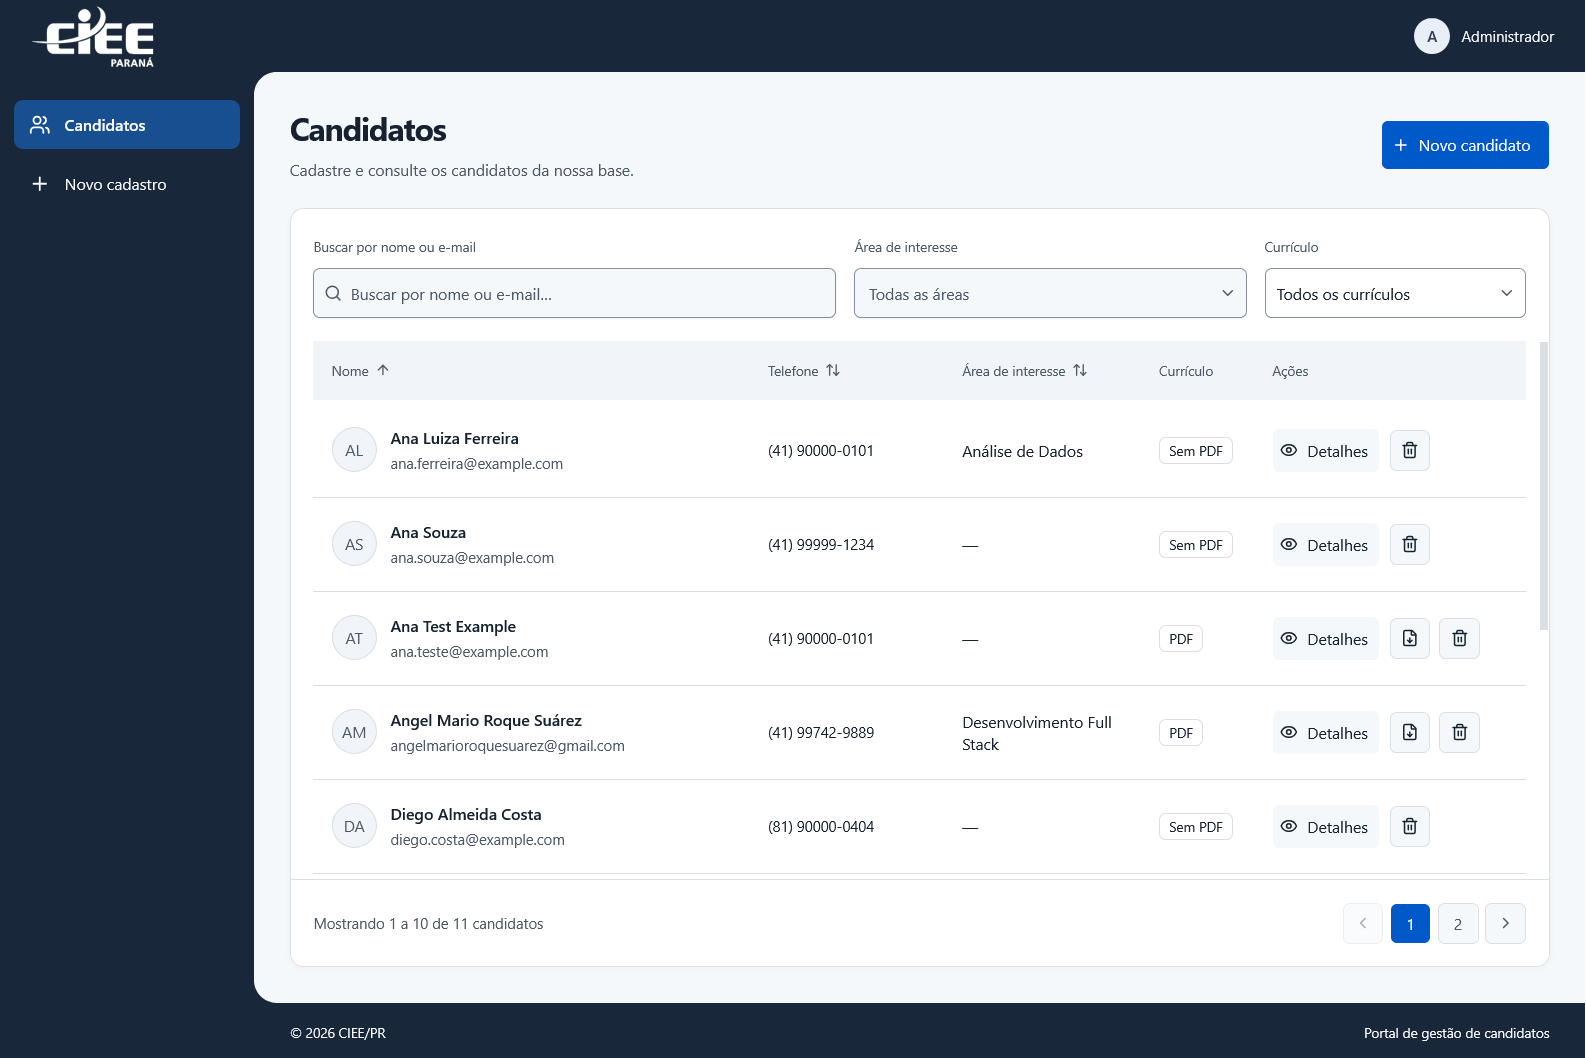
\includegraphics[width=\textwidth]{imagens/interface-listagem.png}
    \vspace{5mm}
    \noindent{\small\color{muted}Interface real da solução: busca, filtros, ordenação e paginação.}
    \vfill

    \noindent{\color{accent}\rule{\textwidth}{1pt}}
    \vspace{4mm}
    \noindent\begin{tabularx}{\textwidth}{Y r}
        \textbf{Angel Mario Roque Suárez}                            & Curitiba -- PR       \\
        Desenvolvedor Fullstack                                      & 3 de outubro de 2026 \\
        React\enspace /\enspace Node.js\enspace /\enspace SQL Server & Versão 1.0.0
    \end{tabularx}
\end{titlepage}
\hypersetup{pageanchor=true}
\pagenumbering{roman}
\pdfbookmark[0]{Sumário}{sumario}
\tableofcontents
\vspace{10mm}
\destaque{Guia de leitura}{%
    Para conhecer a entrega, comece pela visão geral e pelas telas da
    Seção~\ref{sec:interface}. As decisões estão na Seção~\ref{sec:arquitetura};
    os cenários e relatórios, na Seção~\ref{sec:qualidade}.
    O roteiro de avaliação orienta a execução e o anexo reúne os 13 diagramas.}
\clearpage\pagenumbering{arabic}
\section{Visão geral da solução}
Desenvolvi esta aplicação para o desafio técnico de Desenvolvedor de Sistemas
do CIEE/PR. A solução reúne os dois caminhos de cadastro solicitados,
persistência no SQL Server, listagem e consulta de detalhes, com uma
interface integrada à API.

O cadastro manual e o assistido por PDF utilizam o mesmo formulário e as
mesmas validações. A leitura do currículo acontece no backend e retorna
sugestões de nome, e-mail e telefone. O usuário revisa os dados, complementa
as informações e confirma o cadastro. O PDF é opcional em todo o processo.

\destaque{Fluxo principal}{Preencher ou importar\enspace$\rightarrow$\enspace
revisar\enspace$\rightarrow$\enspace salvar\enspace$\rightarrow$\enspace consultar os detalhes.}

\subsection{Melhorias incorporadas}
Além do fluxo central, implementei recursos que facilitam o trabalho de
consulta e organização dos candidatos:
\begin{itemize}
\item busca por nome ou e-mail, filtros por área e presença de currículo;
\item ordenação e paginação, com layout adaptável em tabela ou cartões;
\item armazenamento opcional do PDF e download pela tela de detalhes;
\item exclusão individual com confirmação e operação em lote pela API;
\item e-mail único e normalizado, telefone brasileiro com DDD e confirmação
antes de abandonar alterações do formulário;
\item documentação interativa da API e execução integrada com Docker Compose.
\end{itemize}

\subsection{Tecnologias}
\begin{tabularx}{\textwidth}{P{3cm}Y}
\toprule\cabecalhotabela\textbf{Camada} & \textbf{Tecnologias utilizadas}\\\midrule
Interface & React 19.2.8, TypeScript, Vite 8.2.2, TanStack Router 1.170.32 e TanStack Query 5.104.0.\\
API & Node.js 22+, NestJS 12.0.1 e \texttt{pdf-parse} 2.4.5.\\
Dados & SQL Server 2022, Prisma 7.10.0 e migrations versionadas.\\
Contratos & Zod 4.5.4 compartilhado entre frontend e backend.\\
Arquivos & RustFS compatível com S3 no ambiente local.\\
Workspace & pnpm 11.8.0, Turborepo e Ultracite.\\\bottomrule
\end{tabularx}

\clearpage\section{Atendimento ao desafio}
O quadro relaciona os requisitos do enunciado ao comportamento entregue.
Os diagramas do anexo detalham as operações e suas integrações.

\begin{longtable}{P{4cm}P{\dimexpr\textwidth-4cm-4\tabcolsep\relax}}
\toprule\cabecalhotabela\textbf{Requisito} & \textbf{Solução implementada}\\\midrule\endfirsthead
\toprule\cabecalhotabela\textbf{Requisito} & \textbf{Solução implementada}\\\midrule\endhead
\bottomrule\endfoot
Cadastro manual & Formulário com nome e e-mail obrigatórios e telefone, área e resumo opcionais, sem exigir documento.\\
Cadastro com PDF & Leitura no backend e sugestões para revisão no mesmo formulário do cadastro manual.\\
Revisão dos dados & Campos editáveis antes da confirmação; informações ausentes podem ser preenchidas manualmente.\\
PDF opcional & A falta do arquivo ou falha de leitura mantém o cadastro manual disponível. Guardar o PDF é uma opção separada.\\
Validação & Contratos compartilhados, verificação de e-mail e validação de arquivo PDF com limite de 5.000.000 bytes.\\
Persistência & Cadastro e consultas pela API, com Prisma, SQL Server e migrations para criar a estrutura.\\
Listagem e detalhes & Candidato disponível na listagem após salvar, com acesso a uma tela de dados completos.\\
Mensagens claras & Feedback para validação, arquivo inválido, falha de leitura, cadastro salvo e registro ausente.\\
Configuração e avaliação & README com versões e comandos, exemplos de ambiente, testes e currículo fictício para importação.\\
Registro do trabalho & Relato de decisões, uso de IA, verificações e tempo em \texttt{DESENVOLVIMENTO.md}.\\
\end{longtable}

\subsection{Campos e consistência dos dados}
\begin{tabularx}{\textwidth}{P{4cm}Y}
\toprule\cabecalhotabela\textbf{Campo} & \textbf{Regra aplicada}\\\midrule
Nome completo & Obrigatório; até 200 caracteres, sem aceitar apenas espaços.\\
E-mail & Obrigatório, formato válido, até 254 caracteres; normalizado para minúsculas e único no banco.\\
Telefone & Opcional; telefone brasileiro com DDD, armazenado em dígitos nacionais e apresentado com prefixo +55.\\
Área ou cargo & Opcional; aceita apenas opções da lista predefinida compartilhada entre interface e API.\\
Resumo profissional & Opcional; até 2.000 caracteres.\\\bottomrule
\end{tabularx}

\clearpage\section{Interface e experiência de uso}\label{sec:interface}
Organizei as telas em torno do cadastro e da consulta. A listagem reúne
busca, filtros e ações; o formulário apresenta a importação como auxílio
ao preenchimento; os detalhes agrupam os dados e o acesso ao currículo.
As imagens são capturas da aplicação em execução.

\begin{figure}[H]\centering
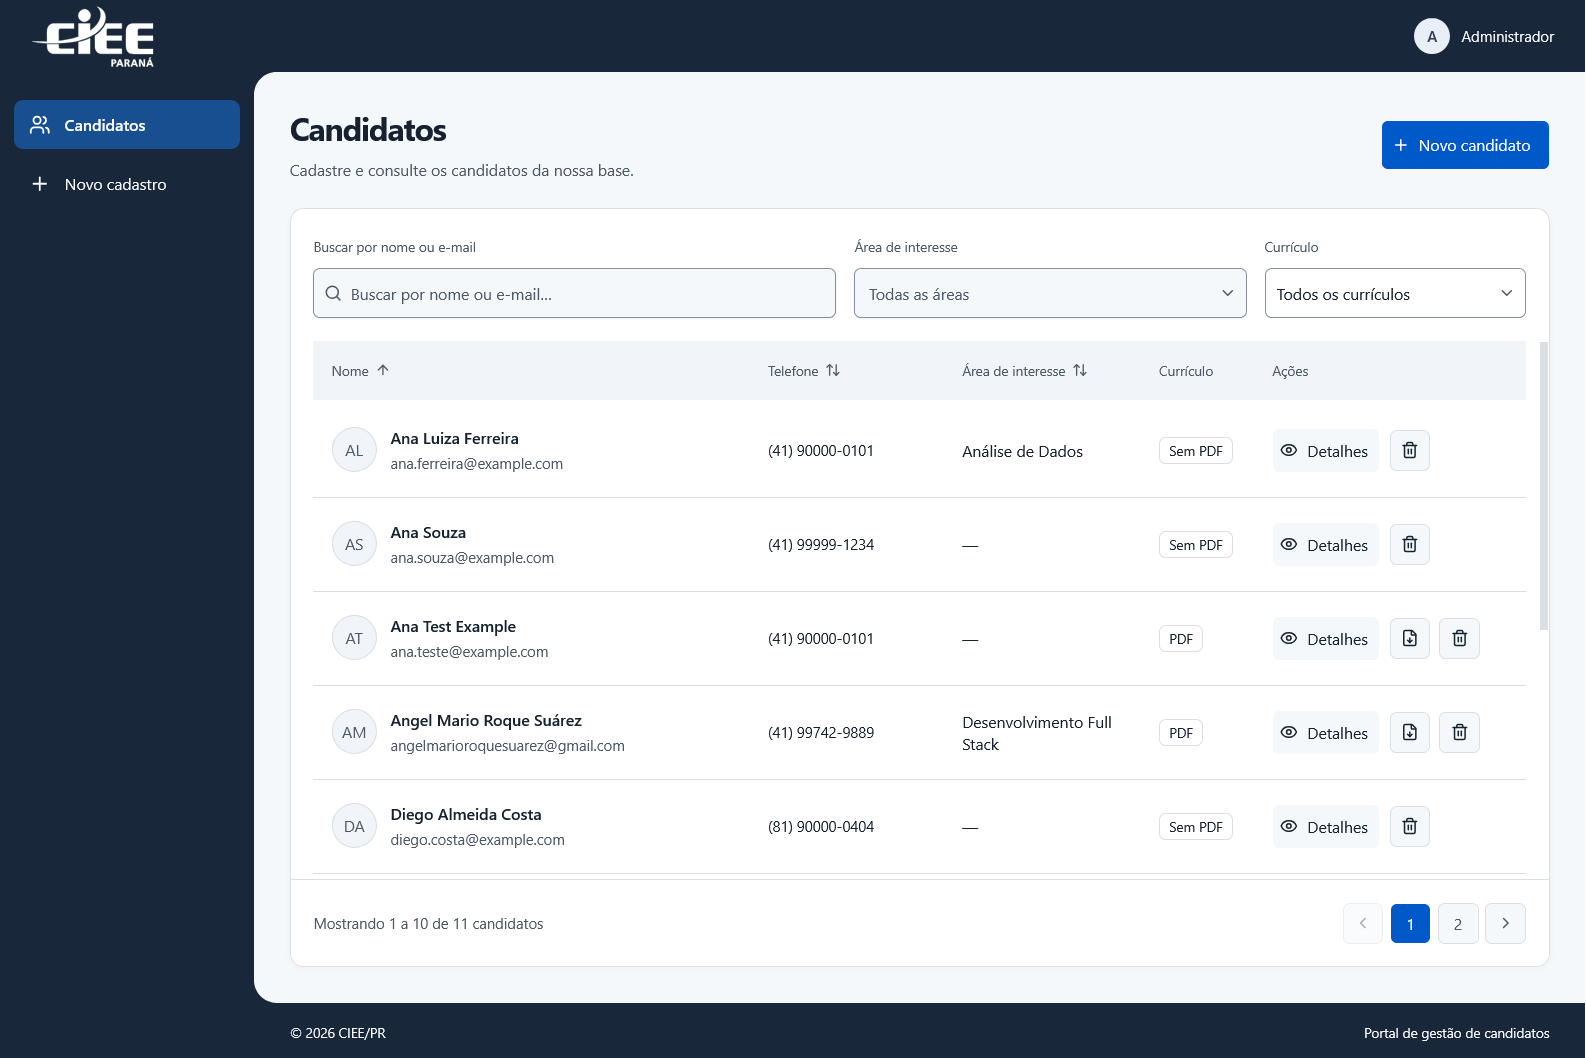
\includegraphics[width=\linewidth]{imagens/interface-listagem.png}
\caption{Listagem com busca, filtros, ordenação, ações e paginação.}
\end{figure}

Os filtros são mantidos na URL, facilitando retornar à consulta. Conforme
o espaço horizontal disponível, os candidatos são apresentados em tabela
ou cartões. A ausência de resultados possui mensagem e ação para limpar a busca.

\telapagina{Cadastro assistido por PDF}
{A importação preenche sugestões no formulário compartilhado. O usuário
confere os campos e escolhe se deseja guardar o arquivo junto ao cadastro.
Após salvar, a interface abre os detalhes do candidato.}
{interface-cadastro.png}
{Formulário com revisão das sugestões e armazenamento opcional do currículo.}

\telapagina{Detalhes do candidato}
{A tela apresenta dados de contato, área de interesse, resumo profissional
e informações do arquivo quando ele foi armazenado. A ação de download
permite acessar o currículo.}
{interface-detalhes.png}
{Dados do candidato e acesso ao currículo na tela de detalhes.}

\clearpage\section{Arquitetura e decisões técnicas}\label{sec:arquitetura}
\subsection{Organização do código}
O monorepo separa a interface em \texttt{apps/web}, a API em
\texttt{apps/backend} e os contratos em \texttt{packages/shared}.
No frontend, componentes e hooks organizam os campos, a importação e a
confirmação. No backend, controllers recebem as requisições e serviços
concentram as operações de candidatos, extração e armazenamento.

\begin{tabularx}{\textwidth}{P{4cm}Y}
\toprule\cabecalhotabela\textbf{Decisão} & \textbf{Motivo e efeito}\\\midrule
Contratos compartilhados & Manter as mesmas regras no formulário e na API, incluindo validação das respostas recebidas.\\
Importação sem persistência & Permitir revisar ou descartar sugestões sem criar registros ou arquivos antecipadamente.\\
Prisma e migrations & Representar o modelo de dados e reproduzir sua estrutura no SQL Server.\\
TanStack Query & Gerenciar consultas, cancelamento e atualização do cache após cadastro ou exclusão.\\
Armazenamento separado & Guardar o PDF em S3/RustFS e manter seus metadados associados ao candidato no banco.\\
Docker Compose & Inicializar os serviços, preparar o armazenamento e aplicar migrations no ambiente de avaliação.\\\bottomrule
\end{tabularx}

\subsection{Modelo de dados}
\texttt{candidates} armazena identificador e os cinco campos do formulário.
\texttt{curriculum\_files} guarda os metadados de zero ou um PDF por candidato:
identificador, referência ao candidato, chave de armazenamento, nome original,
tipo, tamanho e data do upload. A referência ao candidato é única e utiliza
exclusão em cascata dos metadados no SQL Server. O serviço coordena a remoção
do objeto no armazenamento. O e-mail possui restrição única também no banco.

\subsection{Importação, revisão e armazenamento}
O backend valida o limite e a assinatura do PDF e usa \texttt{pdf-parse}
para extrair texto. A resposta contém sugestões, campos ausentes e avisos.
Sugestões encontradas atualizam nome, e-mail e telefone; valores ausentes
preservam o preenchimento atual. Área e resumo são completados manualmente.

O arquivo só acompanha a confirmação se a opção de guardá-lo estiver marcada.
Nesse caso, o backend envia o objeto com uma chave UUID e cria candidato e
metadados com Prisma. Se SQL falhar, tenta remover o upload. O download
retorna uma URL pública do ambiente local, acessada diretamente pelo navegador.

\clearpage\subsection{API e comportamento das operações}
\begin{tabularx}{\textwidth}{P{2cm}P{5.3cm}Y}
\toprule\cabecalhotabela\textbf{Método} & \textbf{Rota sob /api} & \textbf{Operação}\\\midrule
POST & \texttt{/candidates} & Cadastro em JSON ou multipart com PDF opcional.\\
POST & \texttt{/candidates/import-pdf} & Extração de sugestões sem persistência.\\
GET & \texttt{/candidates} & Busca, filtros, ordenação e paginação.\\
GET & \texttt{/candidates/:id} & Dados e metadados do currículo.\\
GET & \texttt{/candidates/:id/}\newline\texttt{curriculum/download} & URL para acessar o arquivo.\\
DELETE & \texttt{/candidates/:id} & Exclusão individual.\\
DELETE & \texttt{/candidates} & Exclusão de até 100 IDs pela API.\\\bottomrule
\end{tabularx}

A busca considera nome ou e-mail. Os filtros incluem área e presença de
currículo. A ordenação aceita identificador, nome, e-mail, telefone ou área.
A paginação usa 10 itens por padrão e até 100 por página; a resposta informa
itens, total e metadados da página. A operação em lote valida e deduplica IDs
e informa a quantidade removida.

\subsection{Tratamento de erros e confirmação}
As operações distinguem dados inválidos (400), registro ausente (404),
e-mail duplicado (409), arquivo grande (413), tipo inválido (415), falha
de leitura (422) e armazenamento indisponível (503). As mensagens permitem
identificar o problema e continuar o cadastro manual quando necessário.

A interface confirma exclusões e a saída de um formulário com alterações.
Ao trocar o PDF, cancela a importação anterior e descarta respostas tardias.
A exclusão remove primeiro o arquivo e depois o registro; a compensação
do upload no cadastro e essa ordem de remoção tratam falhas entre serviços.

\subsection{Ambiente local}
O Compose serve o frontend por Nginx em \texttt{localhost:3001}, a API em
\texttt{localhost:3000}, SQL Server na porta 1433 e RustFS nas portas
9000 (S3) e 9001 (console). A referência interativa da API está em
\texttt{/docs}, com contrato JSON em \texttt{/openapi.json}.
O README descreve a configuração e os comandos para iniciar a stack.

\clearpage\section{Verificação e qualidade}\label{sec:qualidade}
Durante o desenvolvimento, utilizei verificações de tipos, compilação,
lint e formatação, testes unitários e testes e2e da API. A integração
utiliza SQL Server e RustFS reais em um banco dedicado com sufixo
\texttt{\_test}. A suíte cria dados próprios e remove os candidatos que produz.

\begin{tabularx}{\textwidth}{P{4cm}Y}
\toprule\cabecalhotabela\textbf{Grupo de cenários} & \textbf{Verificação realizada no desenvolvimento}\\\midrule
Cadastro e validação & Campos obrigatórios, formatos, normalização, duplicidade e persistência.\\
Importação de PDF & Sugestões, arquivo fictício, campos ausentes, arquivos inválidos e tamanho excedido.\\
Consulta & Listagem, filtros, paginação e consulta de detalhes pela API.\\
Currículo & Upload, download, exclusão e tratamento de falhas entre serviços.\\
Interface & Testes de chamadas da API, cache e hooks; revisão no navegador do formulário e das confirmações.\\
Contrato da API & Schemas OpenAPI de operações e respostas.\\\bottomrule
\end{tabularx}

\subsection{Relatórios de cobertura}
Os relatórios existentes de 3 de outubro de 2026 registram a seguinte
cobertura de linhas. As suítes possuem medições independentes.

\begin{tabularx}{\textwidth}{Y r}
\toprule\cabecalhotabela\textbf{Suíte} & \textbf{Cobertura de linhas}\\\midrule
Backend -- testes unitários & 52,39\%\\
Backend -- integração/e2e & 78,96\%\\
Frontend & 38,35\%\\\bottomrule
\end{tabularx}

As medições incluem fontes não exercitados pelos testes, conforme a
configuração das aplicações. Os arquivos \texttt{coverage-summary.json}
e relatórios HTML permitem conferir os resultados. A automação de
interações completas entre páginas é uma evolução dos testes de frontend,
que hoje cobrem contratos, cache e hooks.

\subsection{Reprodução}
Os comandos de tipos, compilação, lint, testes e cobertura estão no README.
\texttt{QUALIDADE.md} descreve os relatórios; o README do backend explica
a preparação do banco dedicado. Este documento consolida os registros do
desenvolvimento; a revisão editorial não executou novamente as suítes.

\clearpage\section{Processo de desenvolvimento}
\subsection{Planejamento e execução}
Antes da programação, dediquei aproximadamente 2 horas à modelagem no
Visual Paradigm e à preparação do LaTeX. Organizei o trabalho por contratos,
persistência, cadastro, importação, consultas e revisão. Ao final,
dediquei aproximadamente 1 hora à sincronização dos diagramas e da documentação
com a implementação, reunindo os 13 modelos apresentados no anexo.

\subsection{Uso de IA e decisões próprias}
Utilizei Codex no T3 Code, com GPT-6.1-Sol nas sessões registradas, como apoio
à análise, implementação, revisão e documentação. Defini as prioridades e
orientei os ajustes de validação, organização do formulário e comportamento
da aplicação.

Pedidos de unificação das regras resultaram nos contratos compartilhados;
a revisão do formulário ajudou a separar componentes e hooks; a revisão da
API alinhou os testes ao contrato paginado e completou os schemas OpenAPI.
Adaptei as sugestões ao projeto e mantive o formulário com estado React e
validação Zod. O relato completo está em \texttt{DESENVOLVIMENTO.md}.

\subsection{Tempo aproximado}
\begin{tabularx}{\textwidth}{Y r}
\toprule\cabecalhotabela\textbf{Etapa} & \textbf{Tempo}\\\midrule
Modelagem e preparação do LaTeX antes de programar & 2h\\
Desenvolvimento em 02/10: 14h30--17h20 e 19h30--23h & 6h20\\
Desenvolvimento em 03/10: 08h30--12h & 3h30\\
Atualização final dos diagramas e da documentação & 1h\\
Enriquecimento da documentação e revisão final em 03/10: 13h30--14h30 & 1h\\\midrule
\textbf{Total dos períodos registrados} & \textbf{13h50}\\\bottomrule
\end{tabularx}

\subsection{Limites e evolução}
A extração trabalha com texto disponível no PDF. Documentos digitalizados
e layouts ambíguos podem exigir preenchimento manual, como previsto no
desafio. A revisão dos dados permanece disponível em todos os casos.

Com mais tempo, ampliaria a automação das interações da interface e a
reconciliação entre banco e armazenamento. Para um contexto com dados
reais, adotaria controle de acesso e URLs temporárias para os currículos;
o ambiente entregue utiliza acesso direto para avaliação local.

\clearpage\section{Roteiro de avaliação}
\subsection{Executar a aplicação}
Na raiz do repositório, crie \texttt{apps/backend/.env} a partir de
\texttt{apps/backend/.env.example}, configure a senha do SQL Server e execute:

\begin{quote}\ttfamily\small
docker compose --env-file apps/backend/.env up -d --build
\end{quote}

O Compose inicia os serviços, prepara o bucket e aplica as migrations.
Abra \url{http://localhost:3001}. O README também oferece o fluxo de
desenvolvimento local e os comandos de testes.

\subsection{Explorar os dois caminhos de cadastro}
\begin{enumerate}
\item Cadastre um candidato manualmente, sem arquivo, e consulte seus detalhes.
\item Abra um novo cadastro e importe \texttt{examples/curriculo-ficticio.pdf}.
\item Revise as sugestões e complete área e resumo. Marque a opção de
guardar o PDF se desejar experimentar o armazenamento.
\item Salve, consulte os detalhes e acesse o currículo quando armazenado.
\item Volte à listagem e experimente busca, filtros, ordenação e paginação.
\end{enumerate}

\subsection{Materiais para consulta}
\begin{tabularx}{\textwidth}{P{4.6cm}Y}
\toprule\cabecalhotabela\textbf{Material} & \textbf{Conteúdo}\\\midrule
\texttt{README.md} & Visão da aplicação, capturas reais, versões, configuração e comandos.\\
\texttt{DESENVOLVIMENTO.md} & Organização, decisões, participação da IA e tempo dedicado.\\
\texttt{QUALIDADE.md} & Cenários verificados e relatórios de cobertura.\\
\texttt{apps/backend/README.md} & API, ambiente, armazenamento e banco dedicado para testes.\\
\texttt{examples/} & Currículo fictício e exemplos para importação.\\
Anexo deste documento & Casos de uso, arquitetura, dados, implantação e sequências.\\\bottomrule
\end{tabularx}

\destaque{Resultado entregue}{Cadastro manual e assistido por PDF com revisão,
persistência no SQL Server e consulta de candidatos, acompanhado de recursos
de organização, testes e documentação para avaliação.}

\appendix
\clearpage
\section{Diagramas da implementação}
Os modelos foram preparados no Visual Paradigm e atualizados conforme o
desenvolvimento. Este anexo reúne as 13 imagens exportadas do projeto nativo
\texttt{visualp.vpp}. Cada prancha apresenta o propósito do diagrama e o fluxo
correspondente.

\begin{tabularx}{\textwidth}{P{1cm}Y P{3.1cm}}
    \toprule\cabecalhotabela\textbf{ID} & \textbf{Diagrama}             & \textbf{Referência}               \\\midrule
    D01                                 & Casos de uso                  & Figura~\ref{fig:casos}            \\
    D02                                 & Componentes e integrações     & Figura~\ref{fig:componentes}      \\
    D03                                 & Modelo de dados SQL Server    & Figura~\ref{fig:erd}              \\
    D04                                 & Importação e revisão de PDF   & Figura~\ref{fig:importacao}       \\
    D05                                 & Implantação local com Compose & Figura~\ref{fig:implantacao}      \\
    D06                                 & Cadastro manual               & Figura~\ref{fig:cadastro-manual}  \\
    D07                                 & Consulta filtrada e paginada  & Figura~\ref{fig:listagem}         \\
    D08                                 & Consulta de detalhes          & Figura~\ref{fig:detalhes}         \\
    D09                                 & Cadastro com arquivo opcional & Figura~\ref{fig:cadastro-arquivo} \\
    D10                                 & Download do currículo         & Figura~\ref{fig:download}         \\
    D11                                 & Exclusão individual           & Figura~\ref{fig:exclusao}         \\
    D12                                 & Exclusão em lote pela API     & Figura~\ref{fig:exclusao-lote}    \\
    D13                                 & Descarte de alterações        & Figura~\ref{fig:descarte}         \\\bottomrule
\end{tabularx}

\pranchadiagrama{D01 -- Casos de uso}{use-case-diagram.png}
{O usuário cadastra, revisa e consulta candidatos e acessa seus currículos.
O cliente da API também pode realizar exclusões em lote. Os dois caminhos
de cadastro compartilham o formulário e as regras de validação.}{fig:casos}

\pranchadiagrama{D02 -- Componentes e integrações}{component-diagram.png}
{A interface React consulta a API NestJS. Os serviços separam candidatos,
extração de PDF, acesso ao SQL Server com Prisma e operações no armazenamento
S3/RustFS. O navegador acessa diretamente o arquivo ao receber sua URL.}{fig:componentes}

\pranchadiagrama{D03 -- Modelo de dados SQL Server}{database-erd.png}
{Um candidato possui zero ou um arquivo. O e-mail é único e a referência
ao candidato em curriculum\_files também é única. A cascata SQL remove os
metadados; o serviço coordena a remoção do objeto no armazenamento.}{fig:erd}

\pranchadiagrama{D04 -- Importação e revisão de PDF}{pdf-import-sequence.png}
{A API valida e lê o PDF em memória e retorna sugestões, campos ausentes
e avisos. A interface permite revisar o resultado. Essa operação não cria
candidatos nem guarda arquivos, e o cadastro manual continua disponível.}{fig:importacao}

\pranchadiagrama{D05 -- Implantação local com Compose}{deployment-diagram.png}
{O ambiente reúne frontend servido por Nginx, API NestJS, SQL Server e RustFS.
O Compose coordena inicialização do bucket, migrations e volumes. As portas
locais permitem avaliar a interface, a API e o armazenamento.}{fig:implantacao}

\pranchadiagrama{D06 -- Cadastro manual}{manual-registration-sequence.png}
{O formulário envia os dados sem exigir PDF. A API valida, normaliza o e-mail
e persiste o candidato, com proteção contra duplicidade. Após salvar,
a interface atualiza o cache e abre a tela de detalhes.}{fig:cadastro-manual}

\pranchadiagrama{D07 -- Consulta filtrada e paginada}{candidate-list-sequence.png}
{A interface envia busca, filtros, ordenação e parâmetros de página.
O serviço consulta itens e total com os mesmos filtros no SQL Server.
A resposta contém resultados e metadados de paginação.}{fig:listagem}

\pranchadiagrama{D08 -- Consulta de detalhes}{candidate-details-sequence.png}
{A API consulta o candidato e retorna os campos cadastrados e os metadados
do PDF, quando existente. A chave interna de armazenamento não é exposta.
Um registro ausente recebe resposta específica.}{fig:detalhes}

\pranchadiagrama{D09 -- Cadastro com arquivo opcional}{candidate-save-sequence.png}
{Guardar o PDF é uma escolha explícita após revisar os dados. Com arquivo,
o backend faz upload e cria candidato e metadados; se SQL falhar, tenta
remover o objeto enviado. Sem arquivo, o cadastro permanece disponível.}{fig:cadastro-arquivo}

\pranchadiagrama{D10 -- Download do currículo}{curriculum-download-sequence.png}
{O backend verifica candidato e metadados e retorna a URL pública configurada
para o ambiente local. O frontend valida o protocolo HTTP/HTTPS e o navegador
solicita o PDF diretamente ao armazenamento.}{fig:download}

\pranchadiagrama{D11 -- Exclusão individual}{candidate-delete-sequence.png}
{A interface pede confirmação. A API consulta o candidato, remove o arquivo
associado e depois o registro SQL. Uma falha na remoção do arquivo impede
a etapa de exclusão no banco.}{fig:exclusao}

\pranchadiagrama{D12 -- Exclusão em lote pela API}{candidate-bulk-delete-sequence.png}
{A operação valida até 100 IDs, remove duplicatas e considera os candidatos
existentes. O serviço remove seus arquivos antes da etapa SQL e informa
a quantidade excluída. Esse recurso é disponibilizado pela API.}{fig:exclusao-lote}

\pranchadiagrama{D13 -- Descarte de alterações}{discard-changes-sequence.png}
{O formulário confirma a saída quando há alterações. O usuário pode
permanecer ou descartar os dados. Ao desmontar, a interface cancela a
importação ativa; a leitura do PDF não exige limpeza de dados persistidos.}{fig:descarte}

\end{document}
